\documentclass[preview,border=7pt]{standalone}
\usepackage{amsmath,amssymb,xcolor}
\usepackage{tikz}
\usetikzlibrary{arrows.meta}
\definecolor{acc}{RGB}{47,143,132}
\definecolor{cyn}{RGB}{6,182,212}
\definecolor{amb}{RGB}{245,158,11}
\begin{document}
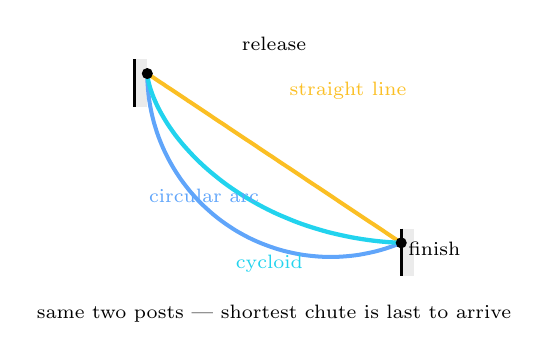
\begin{tikzpicture}
\definecolor{strt}{RGB}{251,191,36}
\definecolor{blu}{RGB}{96,165,250}
\definecolor{cycol}{RGB}{34,211,238}
\fill[black!8] (-0.16,0.18) rectangle (0.00,-0.42);
\draw[line width=1.05pt] (-0.16,0.18) -- (-0.16,-0.42);
\fill[black!8] (3.225, -2.150+0.18) rectangle (3.225+0.16, -2.150-0.42);
\draw[line width=1.05pt] (3.225, -2.150+0.18) -- (3.225, -2.150-0.42);
\draw[strt, line width=1.45pt] plot coordinates {(0.000,0.000) (0.002,-0.001) (0.008,-0.005) (0.018,-0.012) (0.032,-0.022) (0.050,-0.034) (0.073,-0.048) (0.099,-0.066) (0.129,-0.086) (0.163,-0.109) (0.202,-0.134) (0.244,-0.163) (0.290,-0.193) (0.341,-0.227) (0.395,-0.263) (0.454,-0.302) (0.516,-0.344) (0.583,-0.388) (0.653,-0.435) (0.728,-0.485) (0.806,-0.537) (0.889,-0.593) (0.976,-0.650) (1.066,-0.711) (1.161,-0.774) (1.260,-0.840) (1.363,-0.908) (1.469,-0.980) (1.580,-1.053) (1.695,-1.130) (1.814,-1.209) (1.937,-1.291) (2.064,-1.376) (2.195,-1.463) (2.330,-1.553) (2.469,-1.646) (2.612,-1.742) (2.759,-1.840) (2.911,-1.940) (3.066,-2.044) (3.225,-2.150)};
\draw[blu, line width=1.45pt] plot[smooth] coordinates {(0.000,0.000) (0.000,-0.001) (0.000,-0.003) (0.000,-0.006) (0.000,-0.011) (0.000,-0.018) (0.000,-0.026) (0.000,-0.035) (0.000,-0.046) (0.001,-0.058) (0.001,-0.072) (0.002,-0.087) (0.002,-0.103) (0.003,-0.121) (0.004,-0.140) (0.006,-0.161) (0.007,-0.183) (0.009,-0.206) (0.012,-0.231) (0.014,-0.258) (0.018,-0.285) (0.021,-0.315) (0.026,-0.345) (0.031,-0.377) (0.036,-0.410) (0.043,-0.444) (0.050,-0.480) (0.058,-0.517) (0.067,-0.555) (0.077,-0.595) (0.088,-0.636) (0.101,-0.678) (0.114,-0.720) (0.129,-0.765) (0.145,-0.810) (0.163,-0.856) (0.182,-0.903) (0.203,-0.951) (0.225,-0.999) (0.250,-1.049) (0.276,-1.099) (0.304,-1.150) (0.334,-1.201) (0.366,-1.253) (0.400,-1.305) (0.436,-1.357) (0.475,-1.409) (0.516,-1.462) (0.559,-1.514) (0.605,-1.566) (0.653,-1.618) (0.704,-1.669) (0.758,-1.719) (0.814,-1.769) (0.873,-1.818) (0.935,-1.866) (0.999,-1.912) (1.066,-1.957) (1.136,-2.001) (1.209,-2.042) (1.284,-2.082) (1.362,-2.119) (1.443,-2.154) (1.527,-2.186) (1.612,-2.216) (1.701,-2.243) (1.791,-2.266) (1.884,-2.286) (1.980,-2.303) (2.077,-2.315) (2.176,-2.324) (2.277,-2.329) (2.379,-2.329) (2.482,-2.324) (2.587,-2.315) (2.693,-2.301) (2.799,-2.281) (2.906,-2.257) (3.012,-2.227) (3.119,-2.191) (3.225,-2.150)};
\draw[cycol, line width=1.55pt] plot[smooth] coordinates {(0.000,0.000) (0.000,-0.000) (0.000,-0.000) (0.000,-0.000) (0.000,-0.000) (0.000,-0.000) (0.000,-0.000) (0.000,-0.000) (0.000,-0.001) (0.000,-0.001) (0.000,-0.001) (0.000,-0.002) (0.000,-0.003) (0.000,-0.004) (0.000,-0.005) (0.000,-0.006) (0.000,-0.008) (0.000,-0.010) (0.001,-0.013) (0.001,-0.016) (0.001,-0.020) (0.002,-0.024) (0.002,-0.029) (0.003,-0.034) (0.004,-0.041) (0.005,-0.048) (0.006,-0.056) (0.008,-0.065) (0.009,-0.075) (0.012,-0.086) (0.014,-0.099) (0.017,-0.112) (0.021,-0.127) (0.025,-0.143) (0.030,-0.161) (0.036,-0.180) (0.042,-0.201) (0.050,-0.224) (0.058,-0.248) (0.068,-0.274) (0.079,-0.302) (0.091,-0.331) (0.105,-0.363) (0.120,-0.396) (0.137,-0.431) (0.157,-0.469) (0.178,-0.508) (0.202,-0.549) (0.228,-0.593) (0.256,-0.638) (0.288,-0.685) (0.322,-0.734) (0.359,-0.785) (0.400,-0.837) (0.445,-0.892) (0.493,-0.947) (0.545,-1.004) (0.601,-1.063) (0.661,-1.122) (0.725,-1.182) (0.795,-1.243) (0.869,-1.304) (0.947,-1.366) (1.031,-1.428) (1.120,-1.489) (1.214,-1.550) (1.313,-1.609) (1.418,-1.668) (1.527,-1.725) (1.642,-1.780) (1.763,-1.832) (1.888,-1.883) (2.019,-1.930) (2.155,-1.973) (2.295,-2.013) (2.441,-2.048) (2.590,-2.079) (2.743,-2.105) (2.901,-2.126) (3.061,-2.141) (3.225,-2.150)};
\fill (0,0) circle (2.0pt);
\fill (3.225,-2.150) circle (2.0pt);
\node[strt] at (2.55,-0.22) {\scriptsize straight line};
\node[blu] at (0.72,-1.55) {\scriptsize circular arc};
\node[cycol] at (1.55,-2.42) {\scriptsize cycloid};
\node at (1.61,0.38) {\scriptsize release};
\node at (3.225+0.42,-2.150-0.08) {\scriptsize finish};
\node at (1.61,-3.05) {\scriptsize same two posts --- shortest chute is last to arrive};
\end{tikzpicture}
\end{document}
